\section{Schwächen der Textursynthese und deren Verbesserungsmöglichkeiten}

Bisherige Ansätze demonstrieren ihre Algorithmen nur für Beispielmustern mit geringen Auflösungen bis zu $128^2$ Pixeln \cite{SelfTuning}.
Für diese Auflösungen funktionieren die vorgestellten Ansätze gut, denn die entsprechenden Beispielmuster enthalten auf Grund ihrer geringen Größe oftmals nur kleine Details, die sich leicht vervielfachen lassen, ohne dabei unnatscürlich auszusehen.
Höher aufgelöste Beispielmuster leiden dagegen an der \glqq Markov Random Field\grqq -Eigenschaft.
Es werden stets nur kleine lokale Ausschnitte eines Beispielmusters betrachtet, wodurch die globale Ähnlichkeit zu dem benutzten Muster völlig außer Acht gelassen wird.
Folglich werden Texturen aus hochauflösenden Beispielmustern synthetisiert, die den Erwartungen qualitativ hochwertigen Texturen nur selten gerecht werden.

In diesem Kapitel wird eine Textursynthese beschrieben, die sich der Texturoptimierung annimmt und sie mit mehreren Verbesserungen ausstattet, um die bisherigen Probleme der Textursynthese zu überwinden.
Dazu zählen insbesondere das Erhalten von großflächigen Strukturen aus dem Beispielmuster, das Vermeiden von auffälligen Wiederholungen in der synthetisierten Textur und das Erkennen und Bewahren von Regelmäßigkeiten.
Das Verfahren greift dabei Schlüsselideen vorangegangener Verbesserungsmöglichkeiten auf und modifiziert sie in so fern, sodass die Texturoptimierung weiterhin völlig autonom arbeiten kann und keine individuellen, benutzerdefinierten Anpassungen für unterschiedliche Beispielmuster von Nöten sind.

\subsection{Großflächige Strukturen}

Texturen bzw. Beispielmuster enthalten oft Details verschiedener Größen.
So enthält eine Steintextur winzige Details in ihrer Oberfläche, aber wohlmöglich auch größere Strukturen wie etwa Risse oder Kanten.
Diese Strukturen mit großer Ausdehnung werden in der bisherigen Synthese garnicht erst berücksichtigt.

Ein möglicher Ansatz dieses Problem zu lösen ist der Einsatz eines \emph{\glqq Guidance Channels\grqq} \ \cite{SelfTuning}.
Dieser \glqq Guidance Channel\grqq \ erweitert das Beispielmuster um einen zusätzlichen Kanal, in welchem nicht-lokale Informationen über großflächige Strukturen des Beispielmusters gespeichert werden.
\cite{Guidance} zeigt, dass diese Methode besonders gut funktioniert, wenn in ihm die Distanz jedes Pixels zu dem an ihm nächstgelegenen Merkmal (z.B. eine Kontur)  gespeichert wird.
Dieser \glqq Guidance Channel\grqq \ soll im Gegensatz zu bisherigen Verfahren völlig automatisiert berechnet werden und nicht explizit durch den Benutzer übergeben werden müssen \cite{SelfTuning}.

Die Erstellung eines \glqq Guidance Channels\grqq \ umfasst mehrere Schritte, die in Abbildung \ref{Guidance Channel} illustriert sind.

\begin{figure}
	\centering
	\begin{subfigure}{0.3\textwidth}
		\centering
		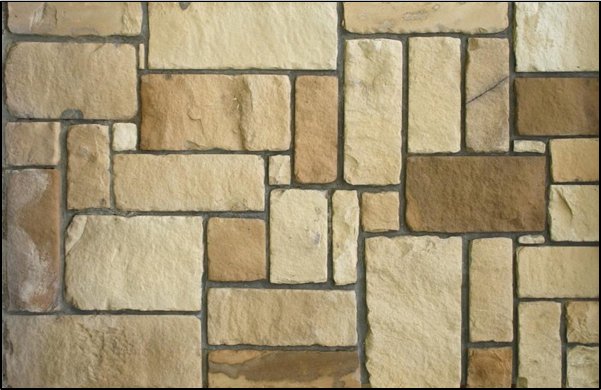
\includegraphics[width=0.8\textwidth]{images/guidance-channel-1}
		\caption{Beispielmuster}
	\end{subfigure}
	\hfill
	\begin{subfigure}{0.3\textwidth}
		\centering
		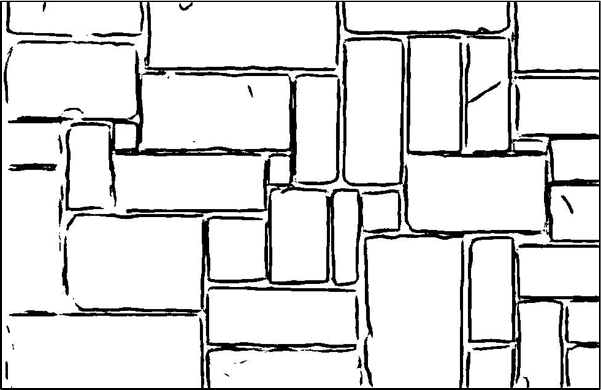
\includegraphics[width=0.8\textwidth]{images/guidance-channel-2}
		\caption{Kantenbild}
	\end{subfigure}
	\hfill
	\begin{subfigure}{0.3\textwidth}
		\centering
		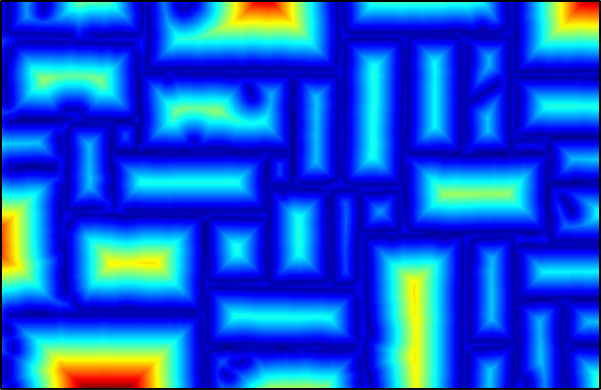
\includegraphics[width=0.8\textwidth]{images/guidance-channel-3}
		\caption{\glqq Guidance Channel\grqq}
	\end{subfigure}
	
	\caption{Erstellung eines \glqq Guidance Channels\grqq \ \cite{SelfTuning}.}
	\label{Guidance Channel}
\end{figure}

Zunächst werden aus dem Beispielmuster Merkmale mit Hilfe eines Kantendetektors extrahiert.
Dies generiert ein graustufiges Kantenbild des Beispielmusters mit kontinuierlichen Werten.
Für die weitere Verarbeitung des Kantenbildes ist dessen Binarisierung nötig.
Mittels Otsus Schwellenwertverfahren (vgl. \cite{Otsu}) wird dazu automatisiert ein optimaler globaler Schwellenwert ermittelt, mit dessen Hilfe das Kantenbild binarisiert werden kann.
Anschließend kann aus dem binarisierten Kantenbild ein Distanzbild bestimmt werden.
Dazu wird mittels MATLABs \texttt{bwdist}-Methode die euklidische Distanz jedes Pixels zu seiner nächstgelegenen Kante berechnet.
Das bedeutet, dass in der Kantenbildmatrix die Distanz von jedem Eintrag mit einer $0$ (keine Kante) zu dem räumlich nächstgelegenen Eintrag mit einer $1$ (Kante) bestimmt wird und in einer neuen Matrix bzw. einem neuen Bild gespeichert wird (dem Distanzbild).
Anschließend wird das Distanzbild entsprechend zum benutzten Farbraum normiert, sodass dessen Werte zu den restlichen Werten des Beispielmusters passen.
Das normierte Distanzbild wird schließlich als \glqq Guidance Channel\grqq \ bzw. als vierter Kanal im Beispielmuster gespeichert (vgl. \cite{SelfTuning}).

Der \glqq Guidance Channel\grqq \ kann schließlich ohne spezielle Anpassung der Texturoptimierung  für die Synthese berücksichtigt werden.
Dazu müssen lediglich die Vektoren $\textbf{t}_p$ und $\textbf{x}_p$ den vierten Kanal für ihre Nachbarschaften mit aufnehmen.
Dann liefert $d(\textbf{t}_p, \textbf{x}_p)$ (vgl. (\ref{nachbarschaftssuche})) ein Ähnlichkeitsmaß zwischen Beispielmuster und Textur unter zusätzlicher Be\-rück\-sich\-ti\-gung des \glqq Guidance Channels\grqq \ \cite{SelfTuning}.

Es zeigt sich jedoch in der Praxis, dass die feste Gewichtung des \glqq Guidance Channels\grqq \ zu Problemen führen kann.
Durch das Hinzufügen eines vierten Kanals verringert sich die Fähigkeit der Synthese, unterschiedliche Materialen bzw. unterschiedliche Farben zwischen einer Kante zu unterscheiden.
Abbildung \ref{Guidance Channel-weight} erklärt dieses Problem anhand eines Beispiels.

\begin{figure}
	\centering
	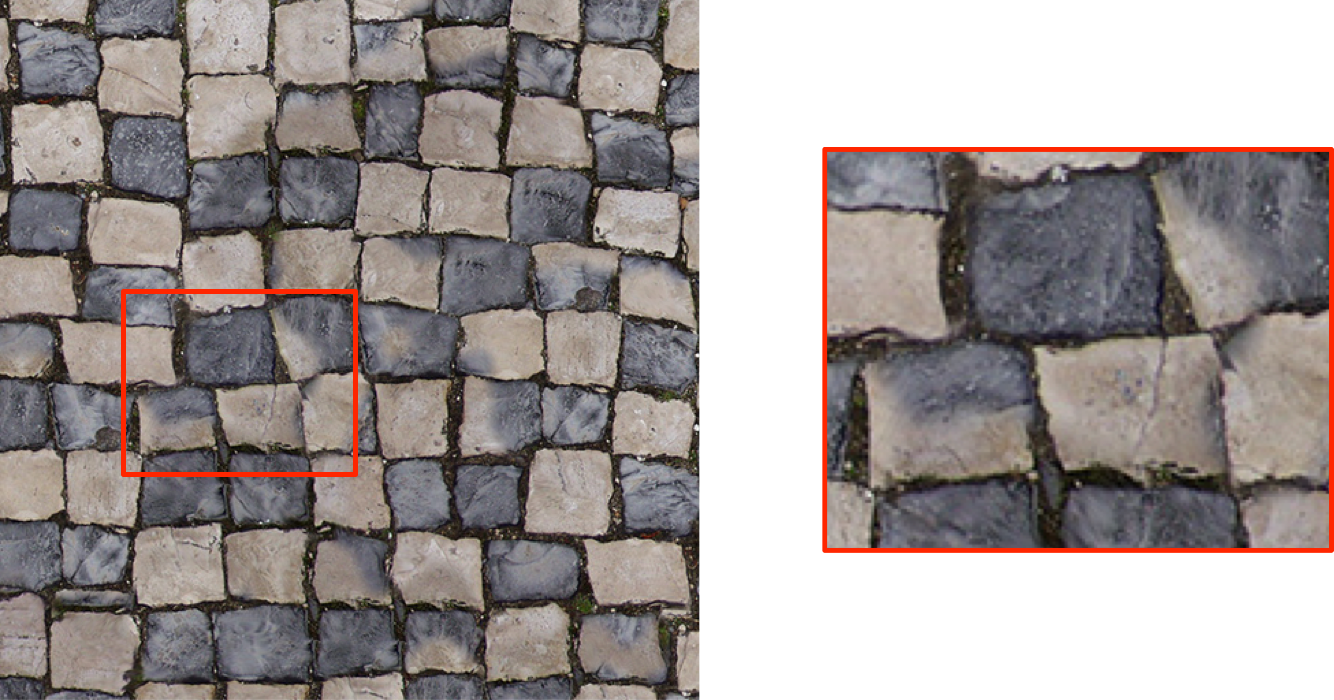
\includegraphics[width=0.5\textwidth]{images/guidance-channel-weight}
	\caption{
		Synthese einer Textur bei fester Gewichtung des \glqq Guidance Channels\grqq \ führt zu schwachen Resultaten bei unterschiedlichen Farbverteilungen an den Kanten.
		Einzelne Kacheln vermischen sich in ihren Farben, da ihr Beitrag zum Gesamtresultat im Vergleich zum \glqq Guidance Channel\grqq \ zu gering ist \cite{SelfTuning}.
	}
	\label{Guidance Channel-weight}
\end{figure}

Um diesem Problem entgegenzuwirken wird eine \emph{adaptive Gewichtung} des \glqq Gui\-dance-Channels\grqq \ genutzt.
Die adaptive Gewichtung ordnet dem \glqq Guidance Channel\grqq \ ein geringeres Gewicht zu, wenn sich die Farben in der räumlichen Nachbarschaft des betrachteten Pixels im Beispielmuster stark unterscheiden.
Damit kann der Vorteil der Berücksichtigung von nicht-lokalen Informationen weiterhin genutzt werden.
Die Gewichtung wird jedoch verringert, falls sie für die Aufrechterhaltung der Qualität der synthetisierten Textur von Nöten ist.

Dazu werden zuerst die Pixelfarben in der direkten Nachbarschaft eines Pixels im Beispielmuster in einer Dichte-Karte gesammelt \cite{SelfTuning}.
Mittels dieser Karte kann schließlich entschieden werden, ob sich die Farben in der betrachteten Nachbarschaft stark unterscheiden.
Dies ist zum Beispiel der Fall, wenn sich mehrere Hügel in der Dichte-Karte wiederfinden.
Unterscheiden sich die Farben nicht, so kann ein hohes Gewicht für den \glqq Guidance Channel\grqq \ gewählt werden.
Andernfalls wird ein etwas zurückhaltenderes Gewicht gewählt \cite{SelfTuning}.

\subsection{Auffällige Wiederholungen}

Bisherige Verfahren garantieren auf Grund der \glqq Markov Random Field\grqq -Eigenschaft nur eine lokale Ähnlichkeit zum Beispielmuster.
Ein kleiner Ausschnitt aus der Textur ist ähnlich zu einem kleinen Ausschnitt des Beispielmusters.
Das führt unmittelbar zu dem Problem, dass sich bestimmte Ausschnitte in der synthetisierten Textur häufig wiederholen, wogegen sich andere Ausschnitte des Beispielmusters nur sehr selten in der Textur wiederfinden.
Zum einen wird dadurch nicht die komplette Vielfalt des Beispielmusters ausgeschöpft und es wird demnach keine globale Ähnlichkeit zum Beispielmuster erreicht werden.
Zum anderen sind für den Betrachter auffällige Wiederholungen in der synthetisierten Textur zu sehen.
Das führt unmittelbar dazu, dass die Ergebnisse der Textursynthese den Anforderungen an eine qualitativ hochwertige Textur nicht gerecht werden.

Zur Lösung dieses Problems können dem Auswahlprozess $\min d(\textbf{t}_p, \textbf{x}_p)$ (vgl. (\ref{nachbarschaftssuche}), (\ref{zielfunktion})) der ähnlichsten Nachbarschaften im Beispielmuster zu den Nachbarschaften in der zu optimierenden Textur bestimmten Einschränkungen (\emph{Constraints}) unterliegen.
\cite{SelfTuning} stellt in diesem Zuge das \emph{\glqq Spatial-Uniformity\grqq} -Constraint vor, mit dem Ziel, eine globale Ähnlichkeit zum Beispielmuster zu garantieren.

Das \glqq Spatial Uniformity\grqq -Constraint soll den Auswahlprozess dazu ermutigen, alle Regionen des Beispielmuster in gleichmäßigem Verhältnis zueinander in der synthetisierten Textur zu berücksichtigen, in dem Regionen bei der Auswahl bestraft werden, die bereits zu oft verwendet wurden.
Damit unterscheidet es sich insbesondere von dem \emph{\glqq Bidirectional Similarity\grqq} -Constraint, welches lediglich garantiert, dass jede Region des Beispielmusters mindestens einmal für die Synthese der Textur benutzt wird (vgl. \cite{BidirectionalSimilarity}) \cite{SelfTuning}.
Für diese Aufgabe wird für jede Iteration der Texturoptimierung eine Vorkommen-Karte $\Omega$ mit

\begin{equation*}
	\Omega(x,y) = \big| \lbrace \textbf{x}_p \ \mid \ (x,y) \in \mathcal{N}(\textbf{x}_p) \rbrace \big|
\end{equation*}
für die Pixel des Beispielmusters aufgebaut, die speichert, wie oft ein Pixel in den Regionen vorkommt, die die Textur bilden.
$\mathcal{N}(\textbf{x}_p)$ kennzeichnet dabei die Menge an Pixeln in der Nachbarschaft um $\textbf{x}_p$ \cite{SelfTuning}.
Abbildung \ref{occurence-map} zeigt die Ausgabe der Vorkommen-Karte $\Omega$ für eine gewöhnliche Textursynthese ohne Constraints.

\begin{figure}
	\centering
	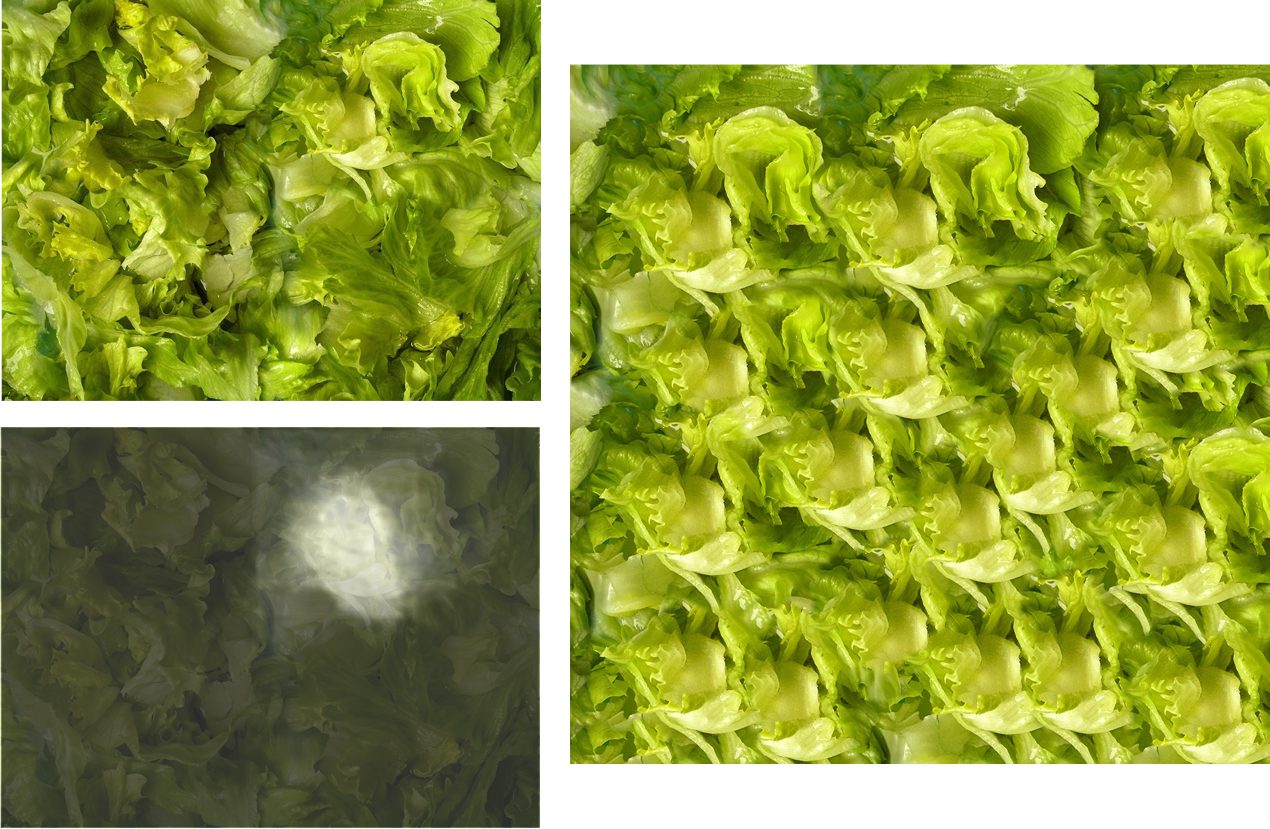
\includegraphics[width=0.5\textwidth]{images/occurence-map}
	\caption{
		Synthese einer Textur ohne Constraints \cite{SelfTuning}.
		Es finden sich auffällige Wiederholungen in der synthetisierten Textur (rechts) wieder.
		Die Vorkommen-Karte $\Omega$ (unten links) des Beispielmusters (oben links) unterstreicht dies, denn es gibt einen deutlich erkennbaren (weißen) Bereich an Pixeln des Beispielmusters, der besonders oft für die Synthese der Textur verwendet wurde.
	}
	\label{occurence-map}
\end{figure}

In einer perfekt balancierten Textur wird jeder Pixel des Beispielmusters gleich oft benutzt.
Die optimale Anzahl dafür wird über

\begin{equation*}
	\omega_{\textit{best}} = \frac{|T|}{|X|}N^2
\end{equation*}
definiert, wobei $|T|$ bzw. $|X|$ die Anzahl der Regionen in $T$ respektive $X$ und $N^2$ die Anzahl der Pixel in jeder Region angeben.

Um den Auswahlprozess zu manipulieren wird der Distanzterm zur Nachbarschaftssuche aus (\ref{nachbarschaftssuche}) modifiziert zu

\begin{equation}
	d(\textbf{t}_p, \textbf{x}_p) = \lVert \textbf{t}_p - \textbf{x}_p \rVert^2 + \lambda \frac{\Omega(\textbf{x}_p)}{\omega_{\textit{best}}}\text{,}
	\label{spatial-similarity}
\end{equation}
wobei $\Omega(\textbf{x}_p)$ den Durchschnitt der globalen Häufigkeit aller Pixel in $\textbf{x}_p$ über

\begin{equation*}
	\Omega(\textbf{x}_p) = \frac{\Sigma_{(x,y) \in \textbf{x}_p}\Omega(x,y)}{N^2}
\end{equation*}
beschreibt.
Formel \ref{spatial-similarity} bestraft damit Regionen $\textbf{x}_p$ umso mehr, je häufiger die Pixel in ihr im Verhältnis zur optimalen Häufigkeit eines Pixels bereits in der synthetisierten Textur vorkommen.
$\lambda = 10$ kontrolliert dabei die Gewichtung des Bestrafungsterms (vgl. \cite{SelfTuning}).

\subsection{Regelmäßigkeiten}

Bisherige Verfahren scheitern daran regelmäßigen oder fast regelmäßigen Strukturen aus dem Beispielmuster korrekt zu reproduzieren.
So ist mit den bisherigen Ansätzen und Verbesserungsmöglichkeiten keinesfalls garantiert, dass Regelmäßigkeiten aus einem Beispielmuster wie etwa Steinkacheln erhalten bleiben.
Das liegt insbesondere an der in Kapitel \ref{chapter-texturoptimierung} erwähnten zufällig generierten Initialisierungstextur \cite{SelfTuning}.
Diese gewährt zwar, dass der Prozess der Synthese mit der korrekten Farbverteilung des Beispielmusters startet, jedoch geht dabei jede globale Struktur, die das Beispielmuster (möglicherweise) aufweist, verloren \cite{SelfTuning}.
Letztendlich kann keine Regelmäßigkeit reproduziert werden, wenn sie im Prozess der Synthese nicht zuvor erkannt wurde.
In der Vergangenheit wurden dazu zahlreiche Ansätze vorgestellt.
\cite{SelfTuning} baut auf diesen Ideen auf und generiert völlig automatisiert eine  Initialisierungstextur, die Regelmäßigkeiten des Beispielmusters wahrt, falls diese vorhanden sind.
Die Texturoptimierung garantiert dann auf Grund der ähnlichsten Nachbarschaftssuche zwischen Beispielmuster und Textur, dass die Regelmäßigkeiten der Initialisierungstextur im weiteren Verlauf der Optimierung erhalten bleiben \cite{SelfTuning}.

\begin{figure}
	\centering
	\begin{subfigure}{0.45\textwidth}
		\centering
		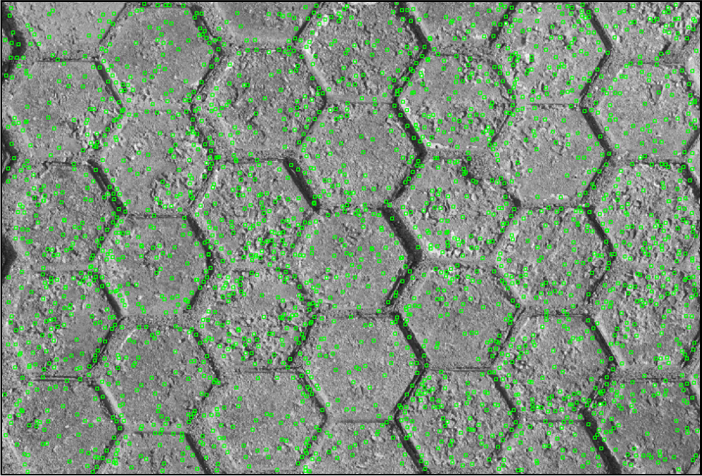
\includegraphics[width=0.7\textwidth]{images/regular-1}
		\caption*{($a$)}
	\end{subfigure}
	\hfill
	\begin{subfigure}{0.45\textwidth}
		\centering
		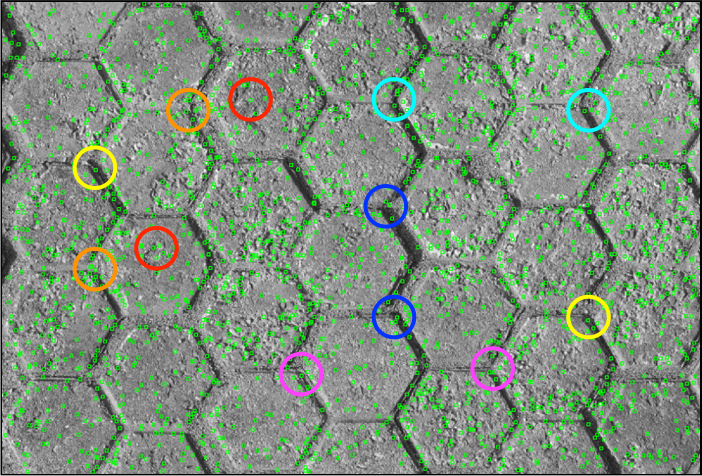
\includegraphics[width=0.7\textwidth]{images/regular-2}
		\caption*{($b$)}
	\end{subfigure}
	\hfill
	\begin{subfigure}{0.45\textwidth}
		\centering
		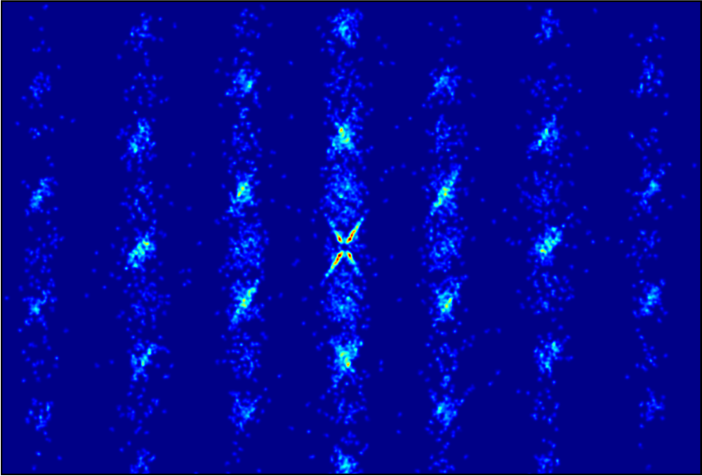
\includegraphics[width=0.7\textwidth]{images/regular-3}
		\caption*{($c$)}
	\end{subfigure}
	\hfill
	\begin{subfigure}{0.45\textwidth}
		\centering
		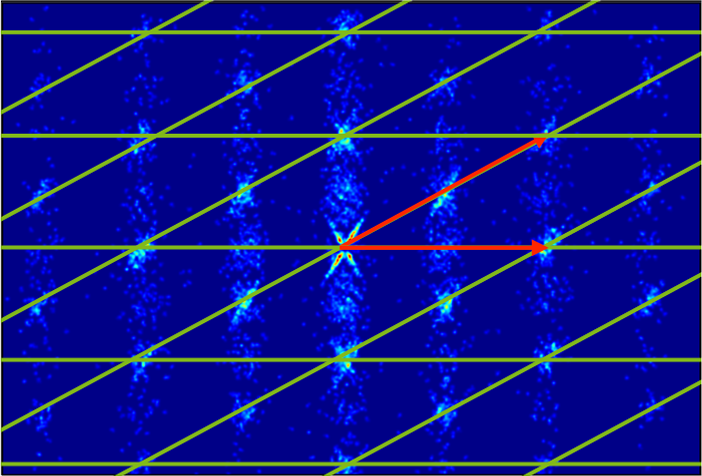
\includegraphics[width=0.7\textwidth]{images/regular-4}
		\caption*{($d$)}
	\end{subfigure}
	
	\caption{
		Berechnung zweier Gitter erzeugender Vektoren \cite{SelfTuning}.
		Zuerst werden die interessantesten Merkmale aus dem Beispielmuster extrahiert ($a$) und eine Menge der ähnlichsten Paare dieser Merkmale bestimmt ($b$).
		Aus den Translationen dieser Paare wird eine Dichte-Karte berechnet ($c$), aus dieser zwei optimale Gitter erzeugende Vektoren ermittelt werden ($d$).
	}
	\label{regular}
\end{figure}

Die Strategie zur Erzeugung der Initialisierungstextur unterteilt sich in zwei Schritte.
Zuerst muss die Regelmäßigkeit des Beispielsmuster gefunden werden.
Dazu sucht man im Beispielmuster nach zwei linear unabhängigen \emph{Gitter erzeugenden Vektoren}, die durch Konkatenation ihrer selbst ein Gitter aufspannen (vgl. Abbildung \ref{regular}$d$).
Anschließend muss auf Basis dieser gefundenen Vektoren die Textur entsprechend initialisiert werden \cite{SelfTuning}.

Abbildung \ref{regular} illustriert den Prozess zur Bestimmung der beiden Gitter erzeugenden Vektoren.
Dazu werden zunächst die interessantesten Merkmalspunkte aus dem Beispielmuster über den \emph{\glqq Difference of Gaussians\grqq} -Algorithmus ermittelt und die SIFT-Deskriptoren für jeden dieser Merkmalspunkte berechnet \cite{SelfTuning}.
Anschließend wird für jedes Merkmal dessen ähnlichstes Merkmal ermittelt.
Dabei werden nur diejenigen Paare für die weitere Berechnung behalten, die sich im Vergleich mit allen Paaren am ähnlichsten sind (vgl. \cite{SelfTuning}).
Für die übrig gebliebenen Paare wird dessen Translation zueinander im Beispielmuster berechnet und in einem zweidimensionalen Koordinatensystem gespeichert.
Aus den Endpunkten dieser Translationen im Koordinatensystem kann dann schließlich eine Dichte-Karte gewonnen werden, die die Häufigkeiten der einzelnen Endpunkte aller Translationen beschreiben.
Hügel in der Dichte-Karte visualisieren dabei auffällige Regelmäßigkeiten von ähnlichen Punkten, die versetzt zueinander sind und die daher als visuelle Regelmäßigkeit im Beispielmuster interpretiert werden können.
Die beiden gesuchten Gitter erzeugenden Vektoren können nun über ein Optimierungsproblem gefunden werden.
Dabei soll das Gitter der beiden Vektoren die Hügel in der Karte optimal beschreiben.
\cite{SelfTuning} bedient sich dafür bei der statistischen Analyse und bestimmt die beiden Vektoren über Maximierung des \emph{\glqq $F_1$-Scores\grqq} (vgl. \cite{F1Score, SelfTuning}) mit

\begin{equation*}
	F_1 = \beta \cdot \frac{\text{Precision} \cdot \text{Recall}}{\text{Precision} + \text{Recall}}\text{.}
\end{equation*}
Dabei beschreibt die \emph{Precision}-Term, in wie weit die beiden Vektoren mit den Hügeln in der Dichte-Karte zusammen passen.
Der \emph{Recall}-Term ermittelt, in wie weit alle Hügel in der Dichte-Karte abgedeckt werden.

Nachdem die Regelmäßigkeit über die Berechnung der beiden Gitter erzeugenden Vektoren ermittelt wurde, kann letztendlich eine Textur initialisiert werden.
Dafür wird das Beispielmuster in disjunkte Bereiche unterteilt, dessen Größe dem umschließenden Rechteck einer Gitterzelle entsprechen.
Diese Bereiche werden dann schließlich sukzessive von links nach rechts und von oben nach unten zufällig in die Textur kopiert \cite{SelfTuning}.

Es zeigt sich, dass die aus dieser Initialisierungsstrategie gewonnenen Texturen Regelmäßigkeiten des Beispielmusters erfolgreich bewahren können.
Insbesondere ist anzumerken, dass diese Initialisierungsstrategie keinen negativen Effekt besitzt, wenn das Beispielmuster keinerlei Regelmäßigkeit aufweist.
Die gefundenen Gitter erzeugenden Vektoren sind in der Regel dann so kurz und die daraus resultierenden disjunkten Bereiche so klein, dass die Strategie in diesen Fällen einer zufälligen Füllung der Textur gleicht (vgl. \cite{SelfTuning}).


